\documentclass[11pt,a4paper]{article}

% ── Pacchetti ──────────────────────────────────────────────────────────────────
\usepackage[T1]{fontenc}
\usepackage[utf8]{inputenc}
\usepackage[italian]{babel}
\usepackage{lmodern}
\usepackage[margin=2.5cm]{geometry}
\usepackage{amsmath,amssymb}
\usepackage{booktabs}
\usepackage{array}
\usepackage{xcolor}
\usepackage{listings}
\usepackage{hyperref}
\usepackage{enumitem}
\usepackage{parskip}
\usepackage{fancyhdr}
\usepackage{microtype}
\usepackage{caption}
\usepackage{graphicx}
\usepackage{setspace}

% ── Colori ─────────────────────────────────────────────────────────────────────
\definecolor{marsred}{RGB}{180,60,40}
\definecolor{codegray}{RGB}{248,248,248}
\definecolor{codecomment}{RGB}{110,110,110}
\definecolor{codestring}{RGB}{160,30,30}
\definecolor{codekeyword}{RGB}{30,80,160}

% ── Stile codice ───────────────────────────────────────────────────────────────
\lstset{
  backgroundcolor=\color{codegray},
  basicstyle=\ttfamily\small,
  breaklines=true,
  commentstyle=\color{codecomment}\itshape,
  keywordstyle=\color{codekeyword}\bfseries,
  stringstyle=\color{codestring},
  numbers=left,
  numberstyle=\tiny\color{gray},
  numbersep=8pt,
  frame=single,
  framerule=0.4pt,
  rulecolor=\color{gray!40},
  tabsize=4,
  language=Python,
  showstringspaces=false,
  captionpos=b
}

% ── Intestazione ───────────────────────────────────────────────────────────────
\pagestyle{fancy}
\fancyhf{}
\lhead{\textcolor{marsred}{\textbf{Mars Rover Exploration Network}}}
\rhead{\textit{Tesina 1}}
\cfoot{\thepage}
\renewcommand{\headrulewidth}{0.4pt}

% ── Titolo ─────────────────────────────────────────────────────────────────────
\title{
  \vspace{-1cm}
  {\Large \textbf{Mars Rover Exploration Network}}\
}
\author{Baris Giorgio \and Fionda Andrea \and Massaro Federico \and Petrilli Davide \\ [0.5cm]
  \small Università degli Studi di Cassino e del Lazio Meridionale\\
  \small Corso di Laurea Magistrale LM-32
}
\date{A.A.\ 2025/2026}

% ══════════════════════════════════════════════════════════════════════════════
\begin{document}
\maketitle
\thispagestyle{fancy}
\tableofcontents
\vspace{0.4cm}
\rule{\linewidth}{0.3pt}
\bigskip

% ══════════════════════════════════════════════════════════════════════════════
\section{Introduzione e specifiche del problema}
\subsection{Introduzione}
La "Space Exploration Agency (SEA)" ha dispiegato una rete di 20 stazioni di esplorazione sulla superficie di Marte. 
Un rover autonomo "Pathfinder-X" deve navigare tra queste stazioni per completare diverse missioni scientifiche, ottimizzando il percorso in base a vincoli specifici per ogni tipo di missione.
Il rover opera in una regione marziara caratterizzata da:
\begin{itemize}
  \item \textbf{Crateri vulcanici}: zone di difficile attraversamento
  \item \textbf{Pianure sabbiose}: zone con alte velocità ma ad alto rischio tempeste
  \item \textbf{Canyon rocciosi}:  zone che offrono protezione ma sono caratterizzate da percorsi tortuosi
  \item \textbf{Altipiani}: zone con buona visibilità ma con alta esposizione alle radiazioni
\end{itemize}
\subsection{Specifiche del problema}
Viene scelta una topologia di rete esagonale che rappresenta la disposizone naturale delle stazioni sulla superficie marziana, con connessioni che riflettono la vicinanza geografica.
All'interno di questa viene considerata una rete di 20 nodi (stazioni di esplorazione), ciascuno con caratteristiche specifiche:
\begin{itemize}
  \item \textbf{Tipo di terreno}: cratere vulcanico, pianura sabbiosa, canyon roccioso o altipiano
  \item \textbf{Radiazione cosmica}: un valore tra 0 e 1 che indica il livello di radiazione al nodo $i$
  \item \textbf{Copertura solare}: un valore tra 0 e 1 che indica la quantità di luce solare disponibile al nodo $i$
  \item \textbf{Visibilità dell'orbiter}: un booleano che indica se il nodo $i$ ha visibilità diretta verso l'orbiter in orbita marziana
\end{itemize}
\begin{table}[h]
\centering
\caption{Caratteristiche dei nodi della rete marziana.}
\small
\begin{tabular}{@{}clllccc@{}}
\toprule
\textbf{ID} & \textbf{Nome} & \textbf{Terreno} & \textbf{Radiazione} & \textbf{Solare} & \textbf{Visibilità} \\
\midrule
0  & Base Camp     & plateau & 0.20 & 0.90 & \checkmark \\
1  & Research Lab  & plateau & 0.30 & 0.85 & \checkmark \\
2  & Crater Edge   & crater  & 0.70 & 0.40 & $\times$   \\
3  & Deep Crater   & crater  & 0.90 & 0.20 & $\times$   \\
4  & North Peak    & plateau & 0.50 & 0.95 & \checkmark \\
5  & Observatory   & plateau & 0.40 & 1.00 & \checkmark \\
6  & Canyon Entry  & canyon  & 0.30 & 0.50 & $\times$   \\
7  & East Ridge    & plateau & 0.60 & 0.80 & \checkmark \\
8  & Dust Plains   & plain   & 0.40 & 0.70 & \checkmark \\
9  & Storm Zone    & plain   & 0.50 & 0.30 & $\times$   \\
10 & Ice Deposit   & plain   & 0.30 & 0.60 & \checkmark \\
11 & South Base    & plateau & 0.20 & 0.85 & \checkmark \\
12 & Ancient River & canyon  & 0.40 & 0.45 & $\times$   \\
13 & Mineral Site  & canyon  & 0.50 & 0.50 & $\times$   \\
14 & Volcanic Vent & crater  & 0.80 & 0.30 & $\times$   \\
15 & Central Hub   & plateau & 0.25 & 0.90 & \checkmark \\
16 & Water Cave    & canyon  & 0.35 & 0.10 & $\times$   \\
17 & West Outpost  & plain   & 0.45 & 0.75 & \checkmark \\
18 & Shelter Bay   & canyon  & 0.20 & 0.40 & $\times$   \\
19 & Crossroads    & plain   & 0.30 & 0.80 & \checkmark \\
\bottomrule
\end{tabular}
\end{table}
Il costo di attraversamentro tra  due nodi dipende dalla distanza tra essi e dal tipo di terreno.

\subsection{Scenari delle missioni}
In questo progetto, il rover deve completare tre missioni distinte, ognuna con obiettivi e vincoli specifici. In questo 
paragrafo andremo a descrivere i tre scenari, evidenziando le differenze chiave e i requisiti di ottimizzazione per ciascuno.
\subsubsection{Scenario 1 -- Scientifico}
Il rover deve partire dal Base Camp (nodo 0) e raggiungere il Mineral Site (nodo 13) minimizzando l'esposizione a radiazioni cosmiche. Il vincolo operativo è che nessun nodo con radiazione superiore a 0.6 può essere attraversato.
La funzione di costo per questo scenario è definita come:
\[
  C_{\text{rad}}(u, v) = d(u, v) \cdot (1 + r_v)
\]
dove $d(u, v)$ è la distanza tra i nodi $u$ e $v$, e $r_v$ è il livello di radiazione al nodo $v$. L'obiettivo è trovare un percorso che minimizzi la somma dei costi di attraversamento, garantendo che tutti i nodi del percorso abbiano $r_i \le 0.6$.
\subsubsection{Scenario 2 -- Rotta solare}
Il rover parte dalla Water Cave (nodo 16) con la batteria quasi scarica e deve raggiungere l'Observatory (nodo 5), che è una stazione di ricarica. L'obiettivo è massimizzare la copertura solare lungo il percorso, con il vincolo che ogni nodo intermedio deve avere copertura solare di almeno 0.5.
La funzione di costo per questo scenario è definita come:
\[
  C_{\text{sol}}(u, v) = d(u, v) \cdot (2.0 - s_v)
\]
dove $s_v$ è la copertura solare al nodo $v$. In questo caso, i nodi con alta copertura solare ($s_v \to 1$) risultano più economici da attraversare, mentre quelli con bassa copertura ($s_v \to 0$) sono penalizzati. L'obiettivo è trovare un percorso che minimizzi la somma dei costi di attraversamento, garantendo che tutti i nodi del percorso abbiano $s_i \ge 0.5$.
\subsubsection{Scenario 3 -- Relay di comunicazione}
Il rover è bloccato nel Deep Crater (nodo 3) senza segnale e deve raggiungere la South Base (nodo 11). Il vincolo operativo è che non si possono attraversare più di 2 nodi consecutivi senza visibilità dell'orbiter.
La funzione di costo per questo scenario è definita come:
\[
  C_{\text{com}}(u, v) = d(u, v) \cdot
  \begin{cases}
    0.8 & \text{se il nodo } v \text{ ha visibilità orbiter} \\
    1.5 & \text{altrimenti}
  \end{cases}
\]
In questo caso, i nodi con visibilità dell'orbiter sono più economici da attraversare, mentre quelli senza visibilità sono penalizzati. L'obiettivo è trovare un percorso che minimizzi la somma dei costi di attraversamento, garantendo che non ci siano più di 2 nodi consecutivi senza visibilità dell'orbiter.

% ══════════════════════════════════════════════════════════════════════════════
\section{Algoritmi utilizzati}

\subsection{A*}

A* è la scelta naturale quando si vuole guidare la ricerca verso il goal in modo intelligente. L'idea centrale è quella di valutare ogni nodo non solo in base a quanto è costato raggiungerlo, ma anche a quanto si stima costerà arrivare al goal da lì:

\[
  f(n) = g(n) + h(n)
\]

dove $g(n)$ è il costo accumulato dal nodo di partenza e $h(n)$ è la stima euristica del costo residuo. Questa combinazione permette ad A* di esplorare preferenzialmente i nodi che sembrano promettenti, evitando di espandere zone del grafo lontane o costose senza motivo.

Nell'implementazione si usa una \texttt{PriorityQueue} (min-heap) per estrarre sempre il nodo con $f$ minima, affiancata da un insieme \texttt{open\_set\_hash} per verificare in tempo costante se un nodo è già in coda. Ogni volta che si trova un percorso più economico verso un nodo già visitato, i punteggi vengono aggiornati e il nodo viene reinserito nella coda.

\begin{lstlisting}[caption={Nucleo del loop A*}]
while not open_set.empty():
    _, current = open_set.get()
    if current == goal:
        return reconstruct_path(came_from, current)
    for neighbor in graph.neighbors(current):
        tentative_g = g[current] + edge_cost(current, neighbor)
        if tentative_g < g.get(neighbor, inf):
            came_from[neighbor] = current
            g[neighbor] = tentative_g
            f[neighbor] = tentative_g + heuristic(neighbor, goal)
            open_set.put((f[neighbor], neighbor))
\end{lstlisting}

Una proprietà importante: se l'euristica è \emph{ammissibile} (non sovrastima mai il costo reale) e \emph{consistente} (soddisfa la disuguaglianza triangolare), A* garantisce di trovare la soluzione ottimale.
Possiamo dire che le funzione euristiche costituiscono l'intelligenza di A*. Ciascuno scenario ha una euristica diversa, costruita per riflettere il criterio di ottimizzazione della missione e per rispettare le proprietà (ammissibilità e consistenza) citate precedentemente.


\subsubsection{Euristica A*: scenario scientifico}
Il rover deve andare dal Base Camp (nodo 0) al Mineral Site (nodo 13) minimizzando l'esposizione a radiazioni cosmiche. Nessun nodo con radiazione superiore a 0.6 può far parte del percorso.

L'euristica è:
\[
  h_{\text{rad}}(n) = d(n,\,\text{goal}) \cdot (1 + r_n)
\]

La motivazione della scelta è la seguente: la distanza euclidea da sola sottostima sempre il costo reale (è ammissibile per costruzione), ma non scoraggerebbe i nodi pericolosi. Moltiplicarla per $(1 + r_n)$ fa sì che i nodi ad alta radiazione risultino ``più lontani'' del necessario, spingendo A* a cercare percorsi alternativi. Poiché $r_n \in [0,1]$, il moltiplicatore non scende mai sotto 1, mantenendo l'ammissibilità.

\subsubsection{Euristica A*: scenario rotta solare}

Il rover parte dalla Water Cave (nodo 16) con la batteria quasi scarica e deve raggiungere l'Observatory (nodo 5), che è una stazione di ricarica. Lungo il percorso, ogni nodo intermedio deve avere copertura solare di almeno 0.5.

\[
  h_{\text{sol}}(n) = d(n,\,\text{goal}) \cdot (2{,}0 - s_n)
\]

Qui la logica è speculare: un nodo con alta copertura solare ($s_n \to 1$) ha un moltiplicatore che si avvicina a 1 -- viene visto come ``vicino'' e quindi preferibile. Un nodo in ombra ($s_n \to 0$) ha moltiplicatore 2, risultando penalizzato. Il fattore 2.0 è scelto per garantire che il moltiplicatore sia sempre positivo e che la funzione rimanga ammissibile anche per $s_n = 0$.

\subsubsection{Euristica A*: scenario relay di comunicazione}

Il rover è bloccato nel Deep Crater (nodo 3) senza segnale e deve raggiungere la South Base (nodo 11). Il vincolo operativo è che non si possono attraversare più di 2 nodi consecutivi senza visibilità dell'orbiter.

\[
  h_{\text{com}}(n) = d(n,\,\text{goal}) \cdot
  \begin{cases}
    0{,}8 & \text{se il nodo ha visibilità orbiter} \\
    1{,}5 & \text{altrimenti}
  \end{cases}
\]

I nodi con segnale vengono resi più ``attraenti'' riducendo la loro stima di costo; i nodi ciechi vengono penalizzati. Il rispetto del vincolo dei 2 hop consecutivi viene verificato esplicitamente dalla funzione \texttt{validate\_communication\_path} dopo la ricerca, che scarta il percorso se il vincolo è violato.
\subsection{BFS}

BFS esplora il grafo a strati concentrici partendo dal nodo di partenza, visitando prima tutti i vicini diretti, poi i vicini dei vicini, e così via. Questo approccio garantisce di trovare il percorso con il minor numero di archi (hop count), ma non tiene conto dei pesi né degli attributi dei nodi.

\begin{lstlisting}[caption={Nucleo del loop BFS}]
queue = deque([start])
visited = {start}
while queue:
    current = queue.popleft()
    for neighbor in graph.neighbors(current):
        if neighbor not in visited:
            visited.add(neighbor)
            came_from[neighbor] = current
            if neighbor == goal:
                return reconstruct_path(came_from, goal)
            queue.append(neighbor)
\end{lstlisting}

BFS ha complessità $\mathcal{O}(V + E)$ garantita, indipendente da qualsiasi euristica. È uno strumento più ``semplice'' rispetto ad A*, ma utile come baseline e in contesti dove la semplicità del percorso (in termini di passi) è davvero ciò che conta.

Il limite principale in questo progetto è che BFS non può integrare direttamente i vincoli ambientali nella ricerca: li ignora durante l'esplorazione, e la validazione avviene solo a posteriori. Questo significa che in alcuni scenari BFS può trovare percorsi validi, ma in altri restituisce soluzioni che non superano i controlli.


% ══════════════════════════════════════════════════════════════════════════════
\section{Confronto tra A* e BFS}
In questo paragrafo ci concentriamo sulle differenze sostanziali tra A* e BFS, evidenziando come queste si manifestano nei tre scenari di missione. Il confronto si basa su diversi aspetti chiave: ottimalità, capacità di integrare vincoli, complessità computazionale e comportamento atteso nei diversi contesti.
\subsection{Differenze degli algoritmi}

\begin{center}
\begin{tabular}{@{}lcc@{}}
\toprule
& \textbf{A*} & \textbf{BFS} \\
\midrule
Ottimale per costo pesato     & \checkmark & \texttimes \\
Ottimale per numero di hop    & \texttimes & \checkmark \\
Integra vincoli nella ricerca & \checkmark & \texttimes \\
Complessità temporale         & $\mathcal{O}(E)$--$\mathcal{O}(V^2)$ & $\mathcal{O}(V+E)$ \\
\bottomrule
\end{tabular}
\captionof{table}{Confronto sintetico tra i due algoritmi.}
\end{center}

\subsection{Differenze nei tre scenari}
% ── Scenario 1 ────────────────────────────────────────────────────────────────
\subsubsection{Scenario scientifico (Base Camp $\to$ Mineral Site).}

\begin{table}[h]
\centering
\caption{Confronto A* vs BFS -- Scenario scientifico.}
\small
\begin{tabular}{@{}lcc@{}}
\toprule
\textbf{Metrica} & \textbf{A*} & \textbf{BFS} \\
\midrule
Criterio di esplorazione      & $f(n) = g(n) + h_{\text{rad}}(n)$ & hop count \\
Vincolo $r_i \leq 0{,}6$      & integrato nell'euristica           & ignorato  \\
Ottimalità sul costo pesato   & \checkmark                         & $\times$  \\
Rischio di invalidazione      & basso                              & alto      \\
Nodi espansi (atteso)         & $\ll V$                            & $\sim V$  \\
\bottomrule
\end{tabular}
\end{table}

A* integra $r_i$ direttamente nella funzione di costo tramite il moltiplicatore $(1 + r_i)$,
penalizzando i nodi ad alto rischio già durante l'esplorazione e orientando la ricerca verso
regioni a bassa radiazione. BFS tratta tutti i nodi come equivalenti e può restituire un
percorso che minimizza gli hop ma viola il vincolo $r_i \leq 0{,}6$ su uno o più nodi
intermedi, risultando non valido dopo la fase di validazione. È lo scenario in cui il
vantaggio qualitativo di A* è più netto.

% ── Scenario 2 ────────────────────────────────────────────────────────────────
\subsubsection{Scenario solare (Water Cave $\to$ Observatory).}

\begin{table}[h]
\centering
\caption{Confronto A* vs BFS -- Scenario solare.}
\small
\begin{tabular}{@{}lcc@{}}
\toprule
\textbf{Metrica} & \textbf{A*} & \textbf{BFS} \\
\midrule
Criterio di esplorazione        & $f(n) = g(n) + h_{\text{sol}}(n)$ & hop count \\
Vincolo $s_i \geq 0{,}5$        & integrato nell'euristica           & ignorato  \\
Preferenza nodi soleggiati      & \checkmark                         & $\times$  \\
Rischio di invalidazione        & basso                              & medio     \\
Nodi espansi (atteso)           & $\ll V$                            & $\sim V$  \\
\bottomrule
\end{tabular}
\end{table}

Il meccanismo è duale rispetto allo scenario precedente: il fattore $(2{,}0 - s_i)$
abbassa il costo stimato dei nodi con alta copertura solare, rendendoli preferibili
durante l'esplorazione. BFS ignora $s_i$ e può produrre percorsi che attraversano nodi
con $s_i < 0{,}5$, fallendo la validazione sugli intermediari. Va notato che, su questa
rete di 20 nodi, la densità degli archi e la distribuzione dei valori solari potrebbero
comunque portare BFS a trovare una soluzione valida: in reti piccole il risultato dipende
fortemente dalla topologia specifica e non è garantito a priori.

% ── Scenario 3 ────────────────────────────────────────────────────────────────
\subsubsection{Scenario di comunicazione (Deep Crater $\to$ South Base).}

\begin{table}[h]
\centering
\caption{Confronto A* vs BFS -- Scenario di comunicazione.}
\small
\begin{tabular}{@{}lcc@{}}
\toprule
\textbf{Metrica} & \textbf{A*} & \textbf{BFS} \\
\midrule
Criterio di esplorazione              & $f(n) = g(n) + h_{\text{com}}(n)$ & hop count \\
Penalità nodi senza visibilità        & fattore $1{,}5$ vs $0{,}8$        & nessuna   \\
Vincolo 2 hop consecutivi ciechi      & orientato dall'euristica           & non gestito \\
Rischio di invalidazione              & basso                              & medio     \\
Nodi espansi (atteso)                 & $\ll V$                            & $\sim V$  \\
\bottomrule
\end{tabular}
\end{table}

Questo è lo scenario in cui il confronto è più sfumato. BFS minimizza per costruzione
il numero di hop, il che implica statisticamente meno nodi ciechi attraversati; tuttavia
non offre nessuna garanzia sul vincolo dei 2 hop consecutivi senza visibilità. A*, guidato
da $h_{\text{com}}$, penalizza i nodi senza segnale con un fattore $1{,}5$ contro $0{,}8$,
orientando attivamente la ricerca verso sequenze di nodi visibili. La validazione
post-ricerca rimane comunque necessaria per entrambi gli algoritmi, poiché né l'euristica
né BFS garantiscono il rispetto del vincolo in senso stretto.
\subsection{Un'osservazione generale}

Il numero di nodi espansi è la metrica più significativa per confrontare l'efficienza dei due algoritmi. A* espande tipicamente molti meno nodi rispetto a BFS, perché scarta presto le direzioni poco promettenti. BFS invece espande tutti i nodi a distanza $k$ prima di procedere al livello $k+1$, indipendentemente da dove si trova il goal. Questa differenza diventa sempre più marcata al crescere della rete.

% ══════════════════════════════════════════════════════════════════════════════
\section{Conclusioni}

Questo progetto mostra concretamente perché la scelta dell'algoritmo di ricerca non è mai neutra: A* e BFS trovano percorsi molto diversi sullo stesso grafo, e la differenza non è solo in termini di costo ma di quali vincoli riescono a rispettare.

A* si è dimostrato più adatto agli scenari con vincoli ambientali continui (radiazione, energia solare), dove la qualità dell'euristica guida la ricerca in modo diretto. Il pattern Strategy adottato per le euristiche si è rivelato la scelta giusta: permette di estendere il sistema a nuovi scenari semplicemente aggiungendo una nuova classe, senza toccare il codice degli algoritmi.

BFS rimane uno strumento valido come baseline e per scenari dove la topologia della rete è tale che il percorso più corto è anche quello più sicuro. La sua semplicità computazionale e l'assenza di parametri da tarare lo rendono una scelta affidabile in contesti meno vincolati.

Un'evoluzione naturale del sistema potrebbe prevedere l'integrazione di \textbf{Dijkstra} come terzo termine di confronto (ottimale per pesi, senza euristica), o approcci basati su \textbf{Reinforcement Learning} per apprendere automaticamente una policy di navigazione adattiva in ambienti dinamici -- un'estensione particolarmente interessante nel contesto di missioni reali su superfici planetarie.

% ══════════════════════════════════════════════════════════════════════════════
\section{Immagini}
\begin{figure}[h]
  \centering
  
\includegraphics[width=0.8\textwidth]{screen/scenario1/s1_iniziale.png}
  \caption{Rappresentazione grafica della rete di stazioni di esplorazione su Marte - scenario scientifico}
\end{figure}
\begin{figure}[h]
  \centering
  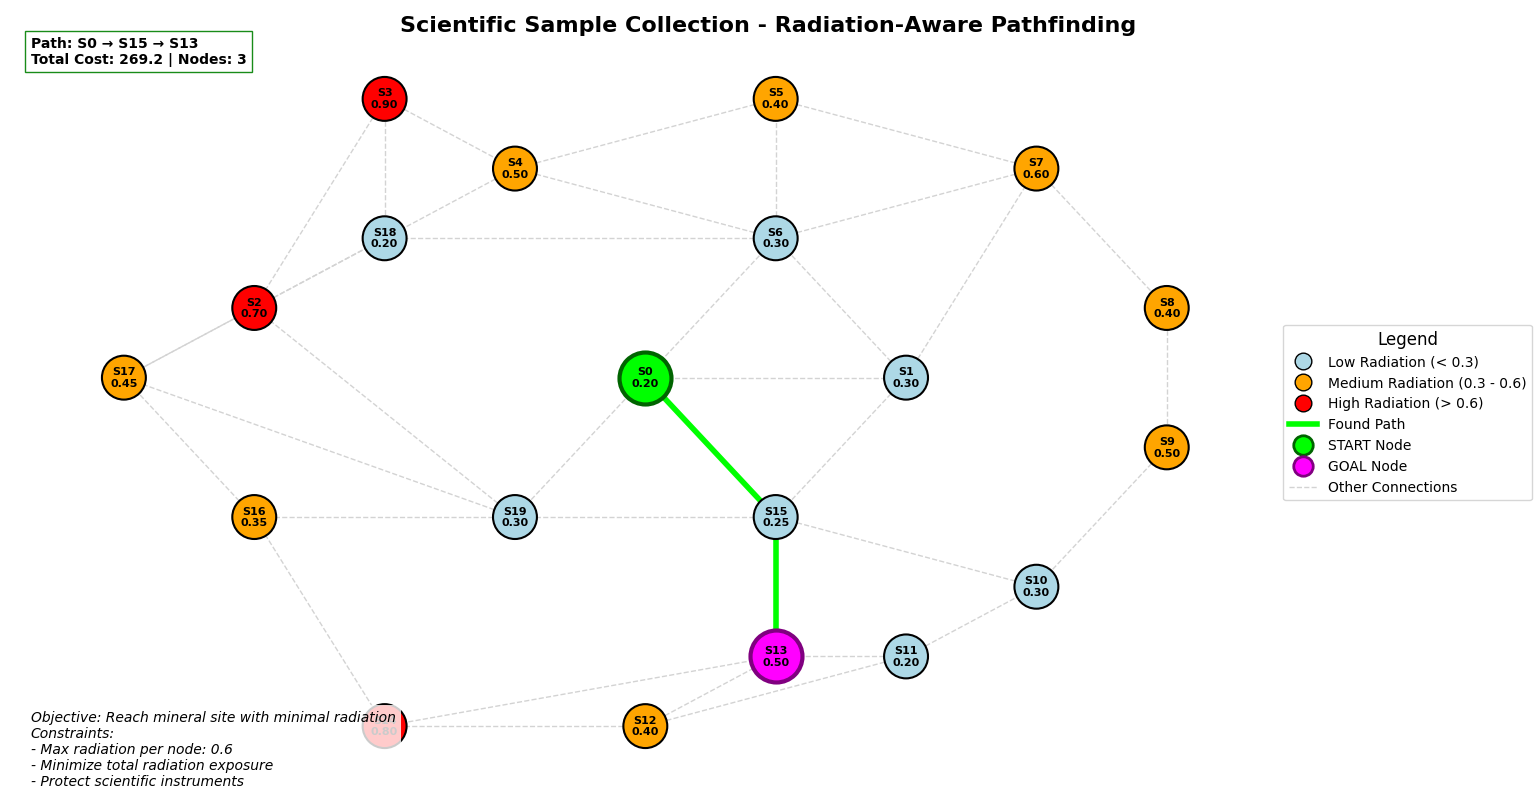
\includegraphics[width=0.8\textwidth]{screen/scenario1/s1_percorso.png}
  \caption{Percorso trovato con algoritmo A* e BFS - scenario scientifico}
\end{figure} 
\begin{figure}[h]
  \centering
  
\includegraphics[width=0.8\textwidth]{screen/scenario1/s1_risultati.png}
  \caption{Recap terminale - scenario scientifico}
\end{figure}

\begin{figure}[h]
  \centering
  
\includegraphics[width=0.8\textwidth]{screen/scenario2/s2_iniziale.png}
  \caption{Rappresentazione grafica della rete di stazioni di esplorazione su Marte - scenario solare}
\end{figure}
\begin{figure}[h]
  \centering
  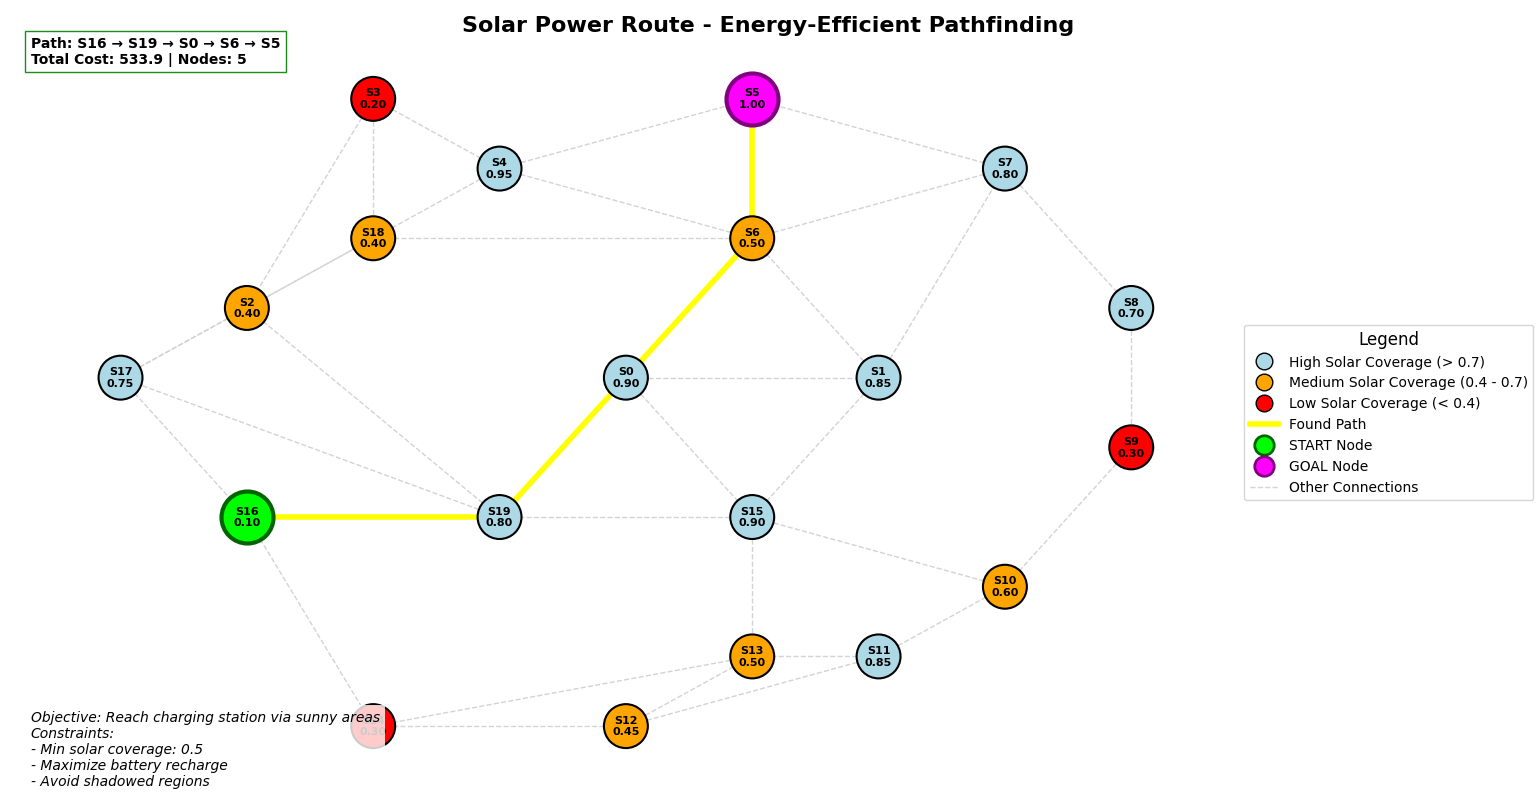
\includegraphics[width=0.8\textwidth]{screen/scenario2/s2_percorso.png}
  \caption{Percorso trovato con algoritmo A* e BFS - scenario solare}
\end{figure}
\begin{figure}[h]
  \centering
  
\includegraphics[width=0.8\textwidth]{screen/scenario2/s2_risultati.png}
  \caption{Recap terminale - scenario solare}
\end{figure}

\begin{figure}[h]
  \centering
  
\includegraphics[width=0.8\textwidth]{screen/scenario3/s3_iniziale.png}
  \caption{Rappresentazione grafica della rete di stazioni di esplorazione su Marte - scenario comunicazione}
\end{figure}
\begin{figure}[h]
  \centering
  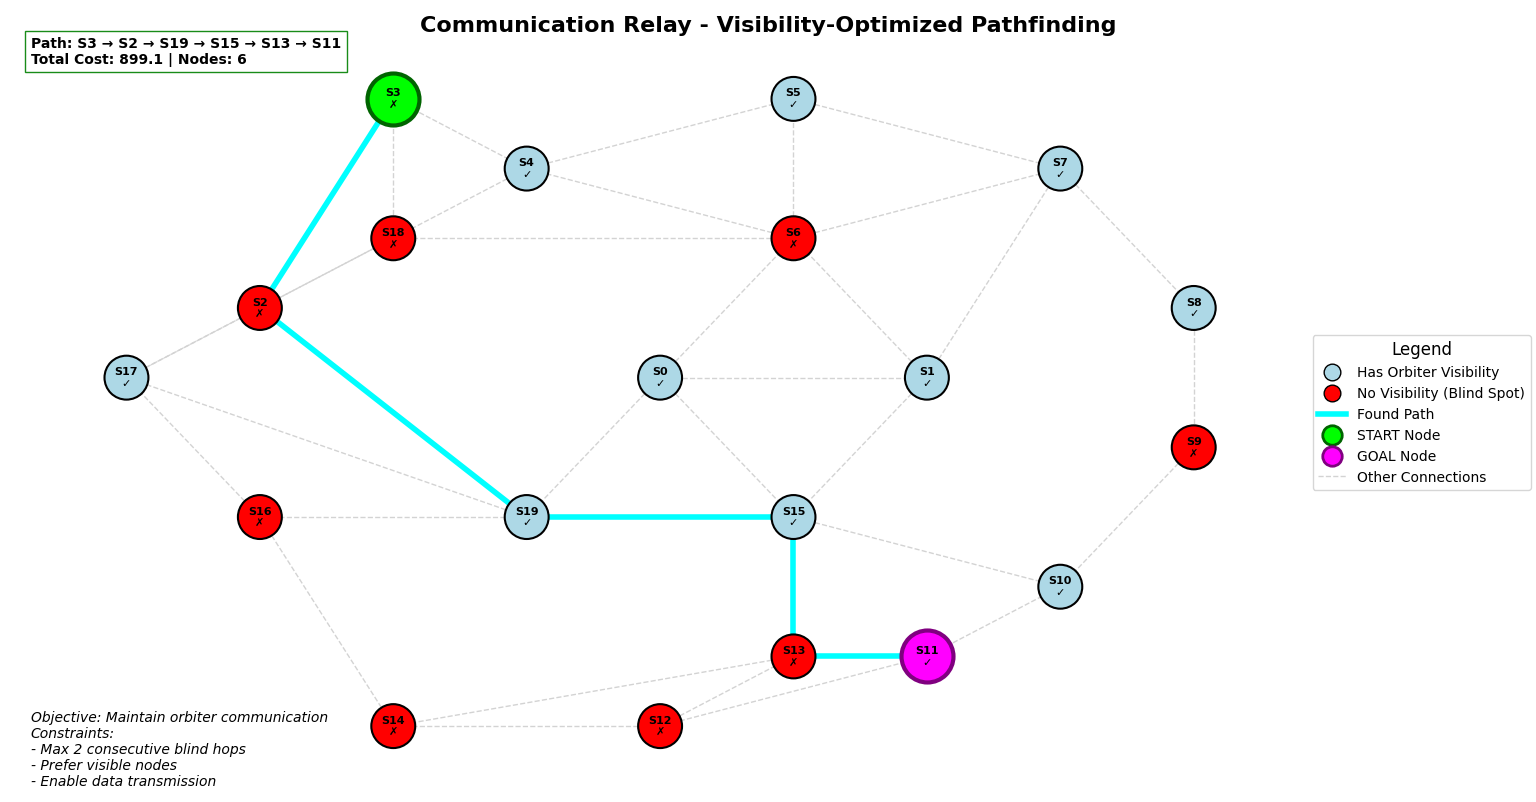
\includegraphics[width=0.8\textwidth]{screen/scenario3/s3_bfs.png}
  \caption{Percorso trovato con algoritmo BFS - scenario comunicazione}
\end{figure}
\begin{figure}[h]
  \centering
  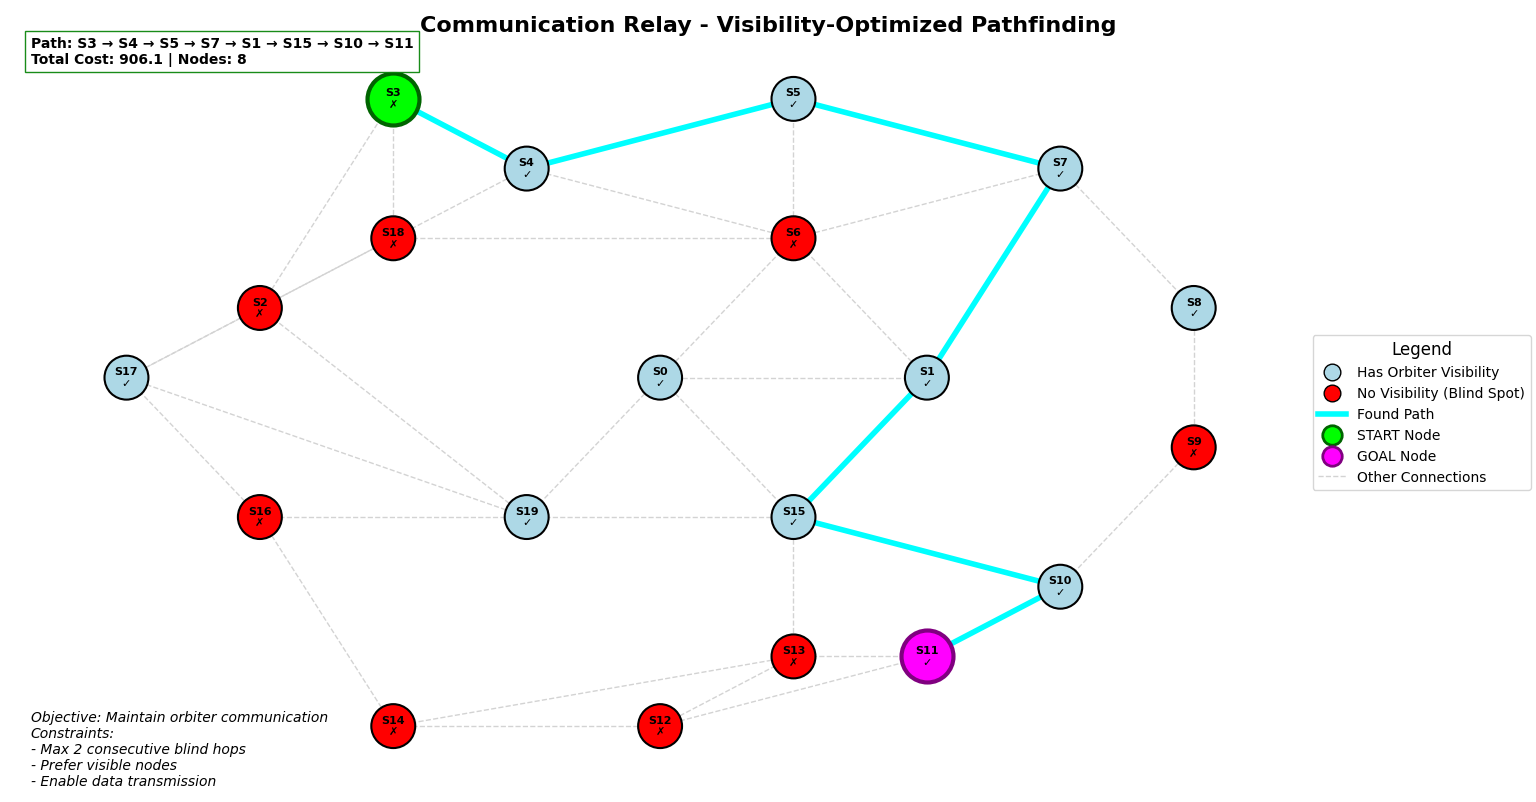
\includegraphics[width=0.8\textwidth]{screen/scenario3/s3_astar.png}
  \caption{Percorso trovato con algoritmo A* - scenario comunicazione}
\end{figure}
\begin{figure}[h]
  \centering
  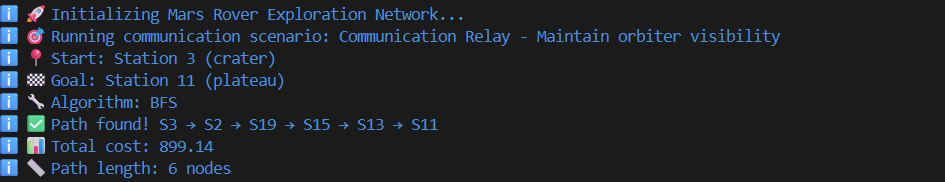
\includegraphics[width=0.8\textwidth]{screen/scenario3/s3_risultati.png}
  \caption{Recap terminale bfs - scenario comunicazione}
\end{figure}
\begin{figure}[h]
  \centering
  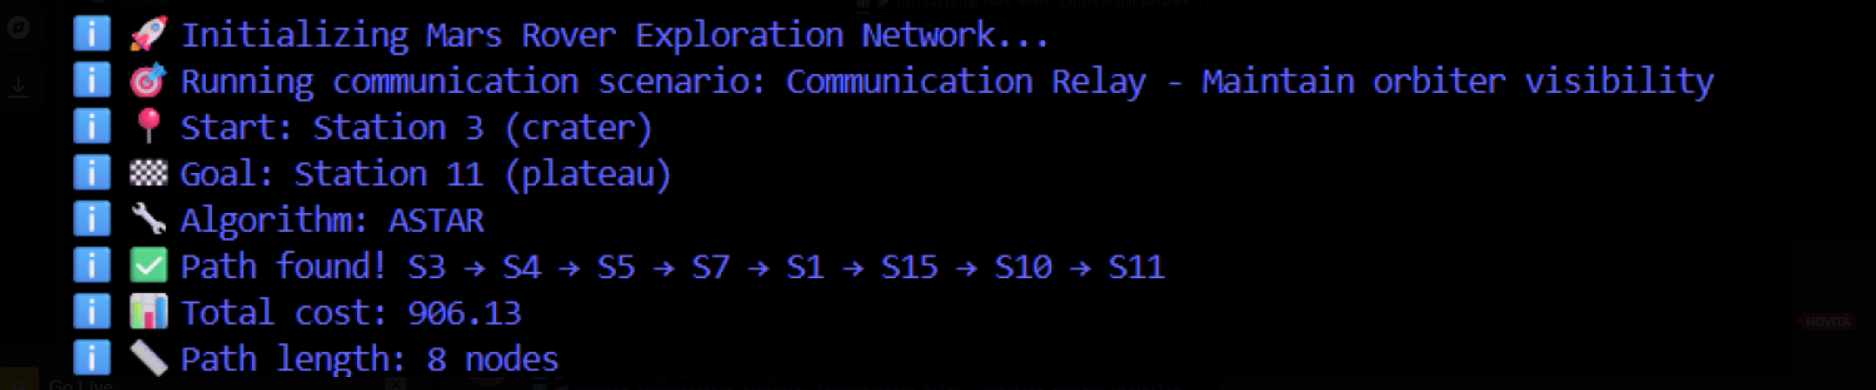
\includegraphics[width=0.8\textwidth]{screen/scenario3/s3_risultatiastar.png}
  \caption{Recap terminale a* - scenario comunicazione}
\end{figure}
\end{document}